\documentclass[a4paper,12pt]{refrep}
\title{Developer Manual}

% Set the page title
\newcommand{\mycontent}[0]{
\begin{tabular}{l}
\hspace*{-4cm} \em XCSoar Developer Manual \vspace*{2pt}
\end{tabular}}

\usepackage{color}
\usepackage{times}
\usepackage{booktabs}
\usepackage{longtable}
\usepackage{rotating}
\usepackage{todonotes}
\usepackage{multirow}
\usepackage{makeidx}\makeindex
\makeatletter
\usepackage{fancyhdr}
\pagestyle{fancy}
\maxipagerulefalse
%
% Include XCSoar header and footer settings and used buttons
\input{xcsoar-headers.sty}
\definecolor{buttongray}{rgb}{0.831,0.816,0.784}
\newcommand{\blink}[0]{$\triangleright$}
\newcommand{\bmenu}[1]{
	\fcolorbox {black}{buttongray}{{\sf{#1}}}
}
\newcommand{\bmenut}[2]{
	\fcolorbox {black}{buttongray}{
    \makebox[1.4cm][c]{
    	\begin{tabular}{c}
    	{\footnotesize\sf{#1}}\\
    	{\footnotesize\sf{#2}}
    	\end{tabular}
    }
  }
}
\newcommand{\bmenuth}[3]{
	\fcolorbox {black}{buttongray}{
    \makebox[1.4cm][c]{
    	\begin{tabular}{c}
    	{\footnotesize\sf{#1}}\\
    	{\footnotesize\sf{#2}}\\
    	{\footnotesize\sf{#3}}
    	\end{tabular}
    }
  }
}
\newcommand{\bmenus}[1]{
	\fcolorbox {black}{buttongray}{
    \makebox[1.4cm][c]{
      \begin{tabular}{c}
        {\footnotesize\sf{#1}}\\
    	  \\
      \end{tabular}
	  }
	}
}
\newcommand{\button}[1]{
	\fcolorbox {black}{buttongray}{{\sf #1}}
}

\newcommand{\infobox}[1]{
	\fcolorbox {black}{white}{\makebox[1.7cm][c]{\sf #1}}
}


\newenvironment{jspecs}{
\itemsep=2pt\topsep=3pt\partopsep=3pt\parskip=0pt
\begin{description}
\itemsep=2pt\topsep=3pt\partopsep=3pt\parskip=0pt
}
{\end{description}}

\newcommand{\jindent}[2]{
  \noindent\makebox[0pt][r]{{#1}\hspace*{\marginparsep}}
  \parbox[t]{0.95\linewidth}{#2}\par
}

%
\widowpenalty=1000
\clubpenalty=1000
%
%  XCSoar - Website Einfügen
\newcommand{\xcsoarwebsite}[0]{\url{www.xcsoar.org}}
%
% Define command to insert tip image
\newcommand{\tip}[0]{\marginlabel{\parbox{1.1cm}{
\includegraphics[width=0.7cm]{figures/reminder.pdf}}}}

% Define command to insert gesture image
%\newcommand{\gesture}[1]{\marginlabel{{\it#1{\phantom{aa}}}\parbox{1.1cm}{\hspace{-3mm}
\includegraphics[width=0.8cm]{figures/gesture.png}}}}
\newcommand{\gesture}[1]{\marginlabel{{\it#1{\phantom{aa}}}\parbox{1.1cm}{\hspace{-3mm}
\includegraphics[width=0.8cm]{figures/gesture.pdf}}}}
%
% Define command to insert warning image
\newcommand{\warning}[0]{\marginlabel{\parbox{1.3cm}{
\includegraphics[width=0.9cm]{figures/warning.pdf}}}}
%
% Define command to insert Achtung image
\newcommand{\achtung}[0]{\marginlabel{\parbox{1.3cm}{
\includegraphics[width=2.5em]{figures/warning.pdf}}}}
%
% Define command to insert a flash image
\newcommand{\blitz}[0]{\marginlabel{\parbox{1.3cm}{
\includegraphics[height=2.0em]{figures/reminder.pdf}}}}
%
% Define command to insert a stop
\newcommand{\halt}[0]{\marginlabel{\parbox{1.3cm}{
\includegraphics[height=2.0em]{figures/warning.pdf}}}}
%
% Define command to reference a configuration item
\newcommand{\config}[1]{\marginlabel{\ref{conf:#1}\parbox{1.3cm}{
\includegraphics[width=0.8cm]{figures/config.pdf}}}}
%
% Potentially overdue ``InfoBox'' style macro
\newcommand{\InfoBox}[0]{{InfoBox}}
%
% Define command to put a menu label on the margin
\newcommand{\menulabel}[1]{\marginpar{\parbox{5.0cm}{\raggedright #1}}}
%
% Define command to draw a sketch on the margin
\newcommand{\sketch}[1]{\marginpar{\parbox{3.750cm}{\includegraphics[angle=0,width=0.9\linewidth,keepaspectratio='true']{#1}}}}
%
% Define command to draw a small sketch on the margin
\newcommand{\smallsketch}[1]{\marginpar{\includegraphics[angle=0,keepaspectratio='true']{#1}}}
%
% Enumerated todo's for the todonotes package
\newcounter{todocounter}
\newcommand{\todonum}[2][]{\stepcounter{todocounter}\todo[#1]{\thetodocounter: #2}}
%
% dies nette Makro bringt mir die aktuelle Version der bearbeiteten XCSoar-Verrion aufs Papier
\newcommand{\version}{\begingroup\catcode`\_=\active\input{VERSION.txt}\endgroup}
%
%Anführungszeichen per Tastatur einfach so eingeben -> "
%\shorthandoff{"}%

\def\maketitle{%
  \null
  \thispagestyle{empty}%
  \begin{maxipage}
    \begin{center}
    
\includegraphics[angle=0,width=0.5\textwidth,keepaspectratio='true']{graphics/logo.pdf}
    \vskip 0.5cm
    
\includegraphics[angle=0,width=0.66\textwidth,keepaspectratio='true']{graphics/title.pdf}
    \end{center}
    \begin{center}
      \normalfont\huge\textsf{La Navigation Open Source}\par
    \end{center}
    \vskip 1cm
    \begin{center}
      \normalfont\huge\textsf{\@title}\par
    \end{center}
    \vskip 1cm
  \end{maxipage}

  \vfill
  \todo[nolist,size=\Large,inline]{Traduction en cours, v�rifiez qu'il n'y a pas de version plus r�cente avant d'imprimer.}

  \begin{flushright}
    \large \strut {
      \sf
      \today \\
      XCSoar version \version \\
      \xcsoarwebsite{} \\
    } 
    \par
  \end{flushright}
  \par
  \vfil
  \vfil
  \null
  \cleardoublepage
}


\usepackage{tikz}
\usetikzlibrary{arrows,shapes,fit,decorations,decorations.pathmorphing,decorations.pathreplacing,calc}

\tikzstyle{thread}=[draw, fill=lightgray, text centered,
  minimum width=7em, minimum height=2.5em]

\begin{document}
\maketitle

\begingroup
\setlength{\parskip}{0.1\baselineskip}
\tableofcontents
\endgroup

%%%%%%%%%%%%%%%%%%%%%%

\chapter*{Preface}

This manual applies to XCSoar version 6.0.  The authors reserve the
right to update this manual as enhancements are made throughout the
life of this product.

\section*{Warnings and precautions}

\warning IT IS THE USER'S RESPONSIBILITY TO USE THIS SOFTWARE PRUDENTLY. THIS
SOFTWARE IS INTENDED TO BE USED ONLY AS A NAVIGATION AID AND MUST NOT
BE USED FOR ANY PURPOSE REQUIRING PRECISE MEASUREMENT OF DIRECTION,
DISTANCE, LOCATION, OR TOPOGRAPHY. THIS SOFTWARE SHOULD NOT BE USED AS
AN AID TO DETERMINE GROUND PROXIMITY FOR AIRCRAFT NAVIGATION.
THIS SOFTWARE SHOULD NOT BE USED AS A TRAFFIC COLLISION AVOIDANCE SYSTEM.


\section*{Legal notices}

\subsection*{Software license agreement}

This software is released according to the GNU General Public License
Version~2.  See Appendix~\ref{cha:gnu-general-public} for the full
text of the agreement and warranty notice.

\subsection*{Limited liability}

In no event shall XCSoar, or its principals, shareholders, officers,
employees, affiliates, contractors, subsidiaries, or parent
organizations, be liable for any incidental, consequential, or
punitive damages whatsoever relating to the use of the Product.

\subsection*{Disclaimer}

This product, and all accompanying files, data and materials, are
distributed "as is" and with no warranties of any kind, whether
express or implied.  This product is used entirely at the risk of the
user.  Although great care has been taken to eliminate defects during
its development it is not claimed to be fault-free. No claims are made
regarding its correctness, reliability or fitness for any particular
purpose.  The XCSoar project developers and contributors shall not be
liable for errors contained herein or for incidental or consequential
damages, loss of data or personal injury in connection with
furnishing, performance, or use of this material.

%%%%%%%%%%%%%%%%%%%%%%%%%%%%%%%%%%%%%%%%%%%%%%%%%%%%%%%%%%%%%%%%

\chapter{Introduction}\label{cha:introduction}

\chapter{Policy}\label{cha:policy}

\section{Writing Patches}

Submit patches or \texttt{git pull} requests to the developer mailing
list (\texttt{xcsoar-devel@lists.sourceforge.net}).  We provide
accounts on \texttt{git.xcsoar.org} to regular contributors.

A patch should be self-explanatory, it needs a good description.  The
subject line specifies the subsystem/library name and a brief
description of what is changed, followed by an empty line.  Then write
a longer description if needed, and explain why this change is needed.

Each patch must compile and must not introduce a regression (as far as
we know at the time).

Each patch must be self-contained and should only change one thing.
Split larger patches into smaller pieces.  Don't refactor and
add/modify/remove features in the same patch.

Don't rewrite code unless you need to.  Migrate incrementally to a new
concept.  Keep patches small and easy to understand.

\section{Code Style}

79 columns, reasonable exceptions allowed.  Indent 2 spaces, no tabs.

\emph{Comments:} write enough code comments (in English).  All
workarounds must be documented.  Everybody must be able to understand
your code, even when you're gone.

\emph{API documentation:} non-trivial functions should be documented
in a doxygen comment.

\emph{Names:} class/function names in \texttt{CamelCase} (not
\texttt{camelCase}); attributes/variables lower case, separated with
underscore (e.g. \texttt{foo\_bar}); constants (including
\texttt{enum} values) all upper case (e.g. \texttt{FOO\_BAR}).

Exception: when a foreign API is being mimicked (e.g. STL containers),
we adopt its naming conventions.

\emph{Files:} \texttt{*.cpp} and \texttt{*.hpp} for C++.  Files should
be named after the main class which is provided.  Each class should
have a separate source file and a separate header.  UNIX text format.

Be \texttt{const}-correct.

Compile with \texttt{WERROR=y} and fix all warnings.

Don't write large functions.  Split them up when they become too
large.

Avoid dynamic allocation.  Dynamic allocation means overhead, more
locking and heap fragmentation.  Use \texttt{StaticArray} and
\texttt{StaticString} if possible.

Asterisks belong to the variable name, not to the type name.  Consider
``\texttt{Foo* a, b}''.  ``\texttt{Foo *a, b}'' or ``\texttt{Foo *a,
  *b}'' is easier to understand.

Some sample code to demonstrate our code style:

\begin{verbatim}
/**
 * API documentation for this class.
 */
struct TheStruct {
  unsigned an_attribute;
  bool second_attribute;

  TheStruct();

  /**
   * API documentation for this method.
   *
   * @param foo documentation for this parameter
   * @return documentation for the return value
   */
  bool TheMethod(int foo);
};

TheStruct::TheStruct()
  :an_attribute(0),
   second_attribute(true)
{
}

static bool
FooBar(int a_parameter, unsigned another_parameter,
       const TheStruct *next_row)
{
  switch (a_parameter) {
  case 0:
    break;
  }

  if (a_parameter == 2 && another_parameter == 3 &&
      next_row != NULL)
    return true;

  return a_parameter == 42;
}
\end{verbatim}

\section{C++}

\subsection{Features}

C++ is a complex language with many features, but some of them come at
a cost (XCSoar runs on weak embedded devices), and others are not
supported well by compilers.  Adopting a new compiler version is
difficult, because the new version may not be available on all
platforms.  This section describes the C++ language features that are
allowed to be used.

XCSoar's standard compiler is \texttt{gcc}.  We need to stay
compatible with version 4.6, because that is what \texttt{cegcc} is
based on.

The following C++ features must \emph{not} be used:

\begin{itemize}
\item RTTI
\item exceptions
\end{itemize}

\subsubsection{C++11}

The XCSoar code base is currently migrating to the new standard
C++11.  The following C++11 features are safe to use:

\begin{itemize}
\item \verb|auto|-typed variables
\item Rvalue references
\item Explicit conversion operators
\item Strongly-typed enums
\item Defaulted and deleted functions
\item Generalized constant expressions (\verb|constexpr|)
\item Range-based \verb|for|
\item \verb|nullptr|
\end{itemize}

\subsection{Other rules}

In a class declaration, attributes come first, then
constructor/destructor, and finally the methods.  Having all
attributes in one place gives a good overview of the nature of a
class.

Avoid expensive and bloated STL containers if there are cheaper
solutions (e.g. \texttt{StaticArray}, \texttt{StaticString} if the
maximum size is predictable).

Avoid template hell.  Keep templates readable.  Keep in mind that
excessive template use may bloat the binary.

\section{Graphical User Interface}
\subsection{Letter Cases}

Following the guidline should prevent the GUI from mixtures of "ON" and 
"On" text elements, and lead to a systematic GUI text presentation. 
The goal is to recognize GUI text fast and reliable.

\begin{description}
  \item[Captions] Captions (button captions, windows titles) to use
        capitalization. E.g. ,"Pan On", "The Display Of ...". 

  \item[Abbreviations] Generally known abbreviation use upper case like "MC", "ETA",
        "V"; or they can use CamelCase, especially when using synthetic
        words  like "GoTo", "InfoBox". 
        Abbreviated words by simply cutting the end of the word needs a
        dot, e.g. "Max. temp."

  \item[Plain text] Longer help texts are to write like prose: "This is the help
        page for ...".

  \item[Labels] Label text has the least systematic constraints:
\begin{itemize}
    \item Captions for text (input) fields, e.g. "Wing loading"
    \item Info text on widgets. E.g. "No data" on an empty
          analysis page. 
    \item Label text for radio or check boxes. 
    \item Selections on Combo-boxes, selectors, Pull-down menus. 
\end{itemize}
  All those should go like prose, whereas exceptions might be
  meaningful.
  
  \item[Gauge caption] Also the appearance of the gauge caption should be covered with
        that. They are currently mapped to upper case all over. I think
        the most readable also here is a CamelCase approach. E.g. to
        distinct "WP Dist", "WP AltD", and "WP AltR". Another good
        example would be MACCREADY, which should be MacCready, or just
        MC.

  \item[Units] Units have their own specific appearance. A profound paper is
        http://physics.nist.gov/cuu/pdf/checklist.pdf we could just
        refer to.
\end{description}


\chapter{Architecture}

This chapter describes XCSoar's internal code architecture.

\section{Source Organisation}

XCSoar's source code is stored in the \texttt{src} directory.  This
section tries to give a rough overview where you can find what.

\begin{itemize}

\item \texttt{Util/}: generic C++ utilities that do not depend on
  external libraries, such as data structures, string operations

\item \texttt{Math/}: math data types (fixed-point math, angles) and
  generic formulas

\item \texttt{Geo/}: geographic data structures and formulas

\item \texttt{Formatter/}: code that formats internal values to
  strings

\item \texttt{Units/}: conversion from SI units (``System'' units) to
  configured user units

\item \texttt{NMEA/}: data structures for values parsed from NMEA

\item \texttt{Profile/}: user profiles, loading from and saving to

\item \texttt{IGC/}: support for the IGC file format

\item \texttt{Logger/}: all loggers (NMEA, IGC, flights)

\item \texttt{Thread/}: multi-threading support (OS specific)

\item \texttt{Screen/}: base library for the graphical user interface

\item \texttt{Renderer/}: various graphical renderers, for map and
  analysis

\item \texttt{MapWindow/}: the map

\item \texttt{Form/}: modal dialogs and their controls (based on the
  screen library)

\item \texttt{Dialogs/}: modal dialogs implementations (based on the
  form library)

\item \texttt{Net/}: networking code (OS specific)

\item \texttt{Operation/}: generic code to support cancellable
  long-running operations

\item \texttt{Android/}: code specific to Android (the native part
  only; Java code is in \texttt{android/src/}

\item \texttt{Engine/PathSolvers/}: an implementation of Dijkstra's
  path finding algorithm, for task and contest optimisation

\item \texttt{Engine/Airspace/}: airspace data structures and airspace
  warnings

\item \texttt{Engine/Waypoint/}: waypoint data structures

\item \texttt{Engine/GlideSolvers/}: a MacCready implementation

\item \texttt{Engine/Task/}: task data structures and calculations

\item \texttt{Engine/Contest/}: contest optimisation

\item \texttt{Engine/Route/}: the route planner (airspace and terrain)

\end{itemize}

\section{Threads and Locking}

\subsection{Threads}

XCSoar runs on multiple threads, to make the UI responsive but still
allow expensive background calculations.

This is how it looks like on Windows and Linux/SDL (software
rendering):

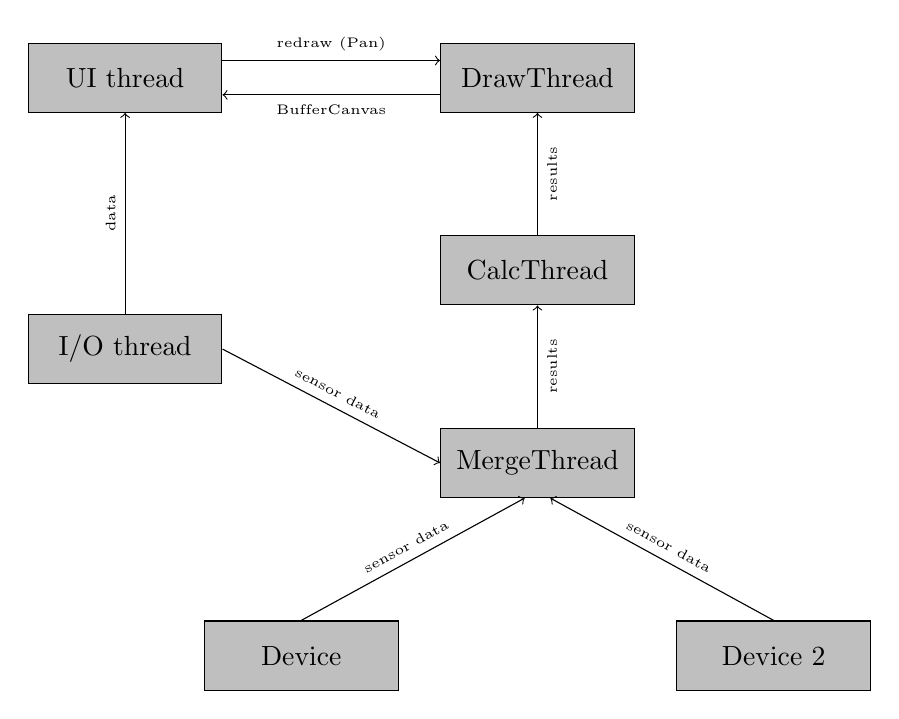
\begin{tikzpicture}
  \node(ui)[thread]{UI thread};

  \path(ui.east)+(4,0) node(draw)[thread]{DrawThread};
  \draw[->] (ui.10) -- (draw.170)
  node[midway, above, sloped, font=\tiny]{redraw (Pan)};
  \draw[->] (draw.190) -- (ui.350)
  node[midway, below, sloped, font=\tiny]{BufferCanvas};

  \path(draw.south)+(0,-2) node(calc)[thread]{CalcThread};
  \draw[->] (calc.north) -- (draw.south)
  node[midway, below, sloped, font=\tiny]{results};

  \path(calc.south)+(0,-2) node(merge)[thread]{MergeThread};
  \draw[->] (merge.north) -- (calc.south)
  node[midway, below, sloped, font=\tiny]{results};

  \path(merge.south)+(-3,-2) node(device1)[thread]{Device};
  \draw[->] (device1.north) -- (merge.250)
  node[midway, above, sloped, font=\tiny]{sensor data};

  \path(merge.south)+(3,-2) node(device2)[thread]{Device 2};
  \draw[->] (device2.north) -- (merge.290)
  node[midway, above, sloped, font=\tiny]{sensor data};

  \path(ui.south)+(0,-3) node(io)[thread]{I/O thread};
  \draw[->] (io.north) -- (ui.south)
  node[midway, above, sloped, font=\tiny]{data};
  \draw[->] (io.east) -- (merge.west)
  node[midway, above, sloped, font=\tiny]{sensor data};
\end{tikzpicture}

The UI thread is the main thread.  It starts the other threads and is
responsible for the UI event loop.  No other thread is allowed to
manipulate windows.  The UI thread has a timer which does regular
house keeping twice per second (\texttt{Pro\-cess\-Ti\-mer.cpp}).

The calculation thread (\texttt{Calcu\-la\-tion\-Thread.cpp},
\texttt{Glide\-Com\-pu\-ter*.cpp}) does all the expensive calculations
in background.  It gets data from the devices (through
\texttt{Merge\-Thread}) and forwards it together with calculation
results to the drawing thread and the main thread.

Each device has its own thread (\texttt{Serial\-Port.cpp}).  This is
needed because Windows CE does not support asynchronous COMM port I/O.
The thread is stopped during task declaration (which happens in the UI
thread).

When new data arrives on the serial port, the \texttt{Merge\-Thread}
gets notified, which will merge all sensor values into one data
structure.  It will then run cheap calculations, and forwards
everything to the \texttt{Calcu\-la\-tion\-Thread}.

With OpenGL, the map is rendered live without a buffer.  There is no
DrawThread.

On Android, the UI thread is not the main thread - the main thread is
implemented in Java, managed by Android itself.  The UI thread listens
for events which the Java part drops into the event queue
(\texttt{NativeView.java} and others).  The internal GPS does not need
a thread, it is implemented with Java callbacks.  For Bluetooth I/O,
there are two threads implemented in Java (\texttt{InputThread.java}
and \texttt{OutputThread.java}, managed by
\texttt{BluetoothHelper.java}).

\subsection{Locking}

Some data structures are rarely modified.  There is no lock for them.
For a modifications, all threads must be suspended.  Example:
waypoints, airspaces.

Other data structures are modified so often that correct locking would
be too much overhead.  Each thread and each instance has its own
copy.  The lock needs to be obtained only for making the private
copy.  The private copy can be used without locking.  Example:
\texttt{NMEA\_INFO}, \texttt{DERIVED\_INFO}.

There are objects which are too expensive to copy.  Normal locking
applies to them.  We have a template class called \texttt{Guard} to
enforce proper read/write locking.  Example: the task.


\section{Accessing Sensor Data}

Much of XCSoar deals with obtaining sensor data and visualising it.

Suppose you want to write a dialog that needs the current GPS
location, where do you get it?  The short and simple answer is: from
\verb|CommonInterface::Basic()| (the \texttt{InterfaceBlackboard}).
Example:

\begin{verbatim}
#include "Interface.hpp"

...
  const auto &basic = CommonInterface::Basic();
  if (basic.location_available)
    current_location = basic.location;
\end{verbatim}

This is true for the main thread (aka the ``user interface thread'').
Other threads must not use the \texttt{Interface.hpp} library, because
the \verb|InterfaceBlackboard| is not protected in any way.  It
contains copies of various data structures just for the main thread.

This is how sensor data moves inside XCSoar:

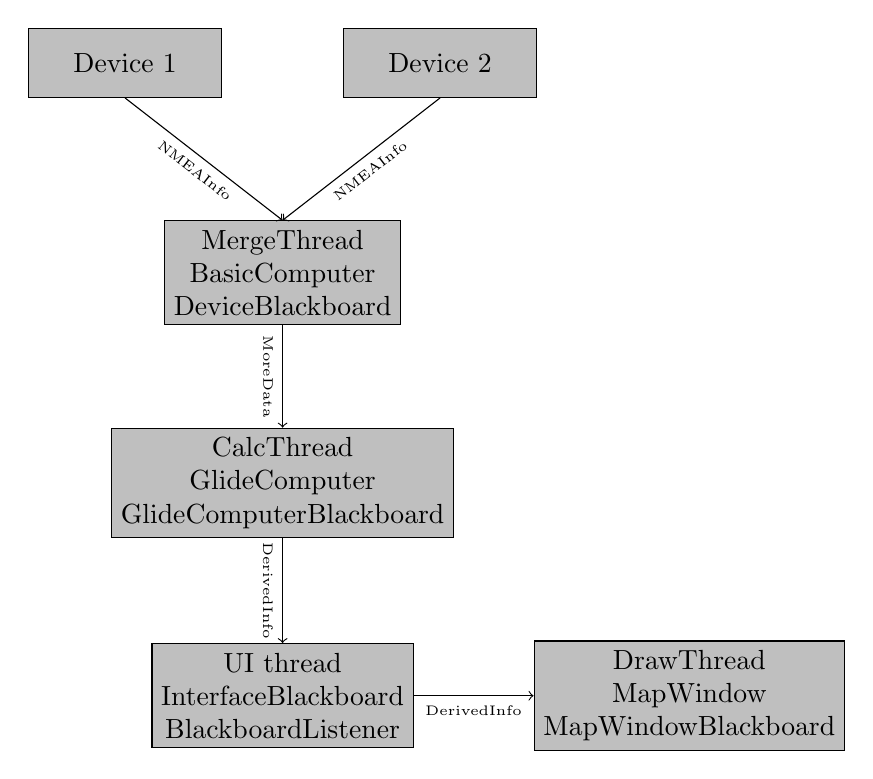
\begin{tikzpicture}
  \node(merge)[thread,align=center]{
    MergeThread\\
    BasicComputer\\
    DeviceBlackboard
  };

  \path(merge.north)+(-2,2) node(device1)[thread]{Device 1};
  \draw[->] (device1.south) -- (merge.north)
  node[midway, below, sloped, font=\tiny]{NMEAInfo};

  \path(merge.north)+(2,2) node(device2)[thread]{Device 2};
  \draw[->] (device2.south) -- (merge.north)
  node[midway, below, sloped, font=\tiny]{NMEAInfo};

  \path(merge.south)+(0,-2) node(calc)[thread,align=center]{
    CalcThread\\
    GlideComputer\\
    GlideComputerBlackboard
  };
  \draw[->] (merge.south) -- (calc.north)
  node[midway, below, sloped, font=\tiny]{MoreData};

  \path(calc.south)+(0,-2) node(ui)[thread,align=center]{
    UI thread\\
    InterfaceBlackboard\\
    BlackboardListener
  };
  \draw[->] (calc.south) -- (ui.north)
  node[midway, below, sloped, font=\tiny]{DerivedInfo};

  \path(ui.east)+(3.5,0) node(draw)[thread,align=center]{
    DrawThread\\
    MapWindow\\
    MapWindowBlackboard
  };
  \draw[->] (ui.east) -- (draw.west)
  node[midway, below, sloped, font=\tiny]{DerivedInfo};
\end{tikzpicture}

The device driver parses input received from its device into its own
\texttt{NMEAInfo} instance inside \texttt{DeviceBlackboard}
(i.e. \verb|per_device_data|).  Then it wakes up the
\texttt{MergeThread} to merge the new data into the central
\texttt{NMEAInfo} instance.  The \texttt{MergeThread} hosts the
\texttt{BasicComputer} which attempts to calculate missing data (for
example, derives vario from GPS altitude).

The \texttt{CalculationThread} wakes up and receives the
\texttt{MoreData} object from \texttt{DeviceBlackboard}.  Here,
expensive calculations are performed (\texttt{GlideComputer}: task
engine, airspace warnings, ...), resulting in a \texttt{DerivedInfo}
object.  The \texttt{CalculationThread} runs no more than twice per
second.

Finally, the UI thread wakes up and receives \texttt{MoreData} and
\texttt{DerivedInfo} via \texttt{DeviceBlackboard}.  This updates
InfoBoxes and other UI elements.  On Windows, the map is drawn in a
separate thread, so there's another layer.

Let's get back to the question: where do I get sensor data?  That
depends on who you are:

\begin{itemize}

\item you are the user interface: (InfoBoxes, dialogs, any Window
  callback): \texttt{InterfaceBlackboard} (see above).  To get
  notified on changes, register a \texttt{BlackboardListener} (and
  don't forget to unregister it).

\item you are the MapWindow: depends!  If you're being called from
  \texttt{OnPaintBuffer} (i.e. inside the \texttt{DrawThread}), you
  must use the \texttt{MapWindowBlackboard}, all others must use the
  \texttt{InterfaceBlackboard}.

\item you are a ``computer'' library: you will get the values as a
  parameter.  Don't try to use the \texttt{GlideComputerBlackboard}
  directly.

\item you are a device driver: implement the method
  \texttt{OnSensorUpdate} or \texttt{OnCalculatedUpdate} if you need
  to know values from other devices or calculation results.

\item everybody else may use the \texttt{DeviceBlackboard}, but be
  sure to lock it while using its data.

\end{itemize}


\chapter{The build system}

A big plain \texttt{Makefile} is used to control the XCSoar build.
GNU extensions are allowed.

\section{Linker parameters}

The following variables (or variable suffixes) appear in the
\texttt{Makefile} (conforming to \texttt{automake} conventions):

\begin{description}
\item[\texttt{LDFLAGS}] Linker flags, such as \texttt{-static} or
  \texttt{-Wl,...}, but not \texttt{-l}.
\item[\texttt{LDLIBS}] All \texttt{-l} flags, e.g. \texttt{-lGL}.
\item[\texttt{LDADD}] Path names of static libraries,
  e.g. \texttt{/usr/lib/libz.a}.
\end{description}

Search directories (\texttt{-L}) are technically linker ``flags'', but
they are allowed in \texttt{LDLIBS}, too.


\chapter{Developing}

\section{Debugging XCSoar}

The XCSoar source repository contains a module for the GNU debugger
(\texttt{gdb}).  It contains pretty-printers for various XCSoar types,
including \texttt{Angle}, \texttt{GeoPoint} and others.  These are
helpful when you print values in the debugger.  To use it, start the
debugging session and load the module:

\begin{verbatim}
$ gdb -ex "source tools/gdb.py" output/UNIX/xcsoar
(gdb) run
\end{verbatim}

The module will automatically convert fixed-point to floating point,
radian angles to degrees and more.  You can now do fancy stuff like:

\begin{verbatim}
(gdb) p basic.location
$1 = GeoPoint(7.93911242887 51.1470221074)
(gdb) p basic.date_time_utc
$2 = DateTime(2012/12/23 21:41:57)
(gdb) p basic.track
$3 = 55.2254197961
(gdb) p basic.external_wind
$4 = GeoVector::ZERO
(gdb) p current_leg.vector_remaining
$5 = GeoVector(267.899420345 107957.109724)
\end{verbatim}



%%%%%%%%%%%%%%%%%%%%%%%%%%%%%%%%%%%%%%%%%%%%%%%%%%%%%%%%%%%%%%%
\chapter{User interface guidelines}

\section{General}

\begin{itemize}
\item Minimise the number of colours, and re-use colour groups already defined.
\item Too much use of colour where it is not required serves only to reduce 
 the effectiveness of bright colours for important items.
\item High colour saturation elements should be reserved for high importance items
\item High contrast against background should be reserved for high importance items
\item Attempt to adopt colours that are intuitive based the function of the item
\item Minimise the clutter where possible --- readibility is essential for use 
 in flight
\item Use colours defined in \verb|Graphics| according to functional name, not 
 their actual colour.
\item Try to maintain consistent use of colours in all uses of that function, 
 such as dialogue graphics as well as map overlays and infoboxes.
\item Text should always be monochrome.
\end{itemize}

Use aviation conventions or adopt best aviation human factors
standards where possible, in particular:
\begin{itemize}
\item ICAO Internation Standards and Recommended Practices, Annex 4 to the 
 Convention on International Civil Aviation (Aeronautical Charts).
\item NASA Colour Usage recommendations and design guidelines: \verb|http://colorusage.arc.nasa.gov/|
\item DOT/FAA/AR-03/67 {\em Human Factors Considerations in the Design and 
 Evaluation of Electronic Flight Bags (EFBs)} \verb|http://www.volpe.dot.gov/hf/aviation/efb/docs/efb_version2.pdf|
\item FAA Human Factors Design Standards \verb|http://hf.tc.faa.gov/hfds/|.
\item DOT/FAA/AM-01/17 {\em Human Factors Design Guidelines for Multifunction Displays}
\end{itemize}

Check for performance with respect to colour blindness.
This site has a useful tool that can be used to convert screenshots
to how they would look to a person with common color blindness:
\verb|http://www.etre.com/tools/colourcheck/|.

{\bf For safety purposes, avoid use of elements that may encourage or require 
the user to stare at the screen continuously.}

{\bf For safety purposes, avoid user controls that have significant risk of 
producing unsafe results if misconfigured by the pilot.}

\subsection{General colour conventions}
Colour conventions generally in use throughout the program:
\begin{itemize}
\item Red for indicator of warning
\item Orange for indicator of caution
\item Green for positive indicator of safety
\item Blue for neutral indicator of safety
\end{itemize}

\subsection{Displayed data}
\begin{itemize}
\item Where data is invalid, indicate this by not presenting the data or
  showing dashes.
\item Present data in user-defined units.
\item Display numerical data with significant digits appropriate to the accuracy of the
  calculations, or its functional use by the pilot, whichever is lower.
\end{itemize}

\section{Dialogs and menu buttons}

\subsection{Colors}
Colour conventions in use are:
\begin{itemize}
\item Grey for buttons
\item Buttons and other widgets rendered with an evenly shaded border
\item Yellow for clicked items
\item Light blue for the key focused item
\item Medium blue for dialogue title bar
\item Text is black if the item is enabled
\item Text is greyed out (but still visible) if the item is disabled
\end{itemize}

\subsection{dialogue types and navigation buttons}
There are four types of dialogs in XCSoar, and the navigation 
buttons for each are different.  
Navigation buttons are the Close, OK, Cancel and Select buttons.
\begin{itemize}
\item Dialogs that modify and save data when the dialogue closes.

These shall usually have a Close button (no Cancel) and may have context specific 
function buttons
\item Dialogs that modify data where Cancel would be important for the user.

These shall have OK and Cancel buttons.  This may include dialogs with 
children dialogs where hitting Cancel from the parent dialogue cancels 
all the changes made in the children dialogs

\item Dialogs that have a list of values, one of which can be selected to 
 return to the parent dialogue.

These shall have Select and Cancel buttons
\item Dialogs that display information that cannot be modified.

These shall have a Close button
\end{itemize}

\subsection{dialogue button placement and size}
\begin{itemize}
\item The Close and Cancel buttons will never appear in the same dialogue and 
 are always located in the same place.  This location will be:

For portrait: lower right

For landscape: lower left
\item The Select button will be accompanied with a Cancel button.  The locations will be:

For portrait: Select in lower left, Cancel in lower right

For landscape: Cancel in lower left, Select immediately above it
\item Buttons will be 35 (scaled) pixels high
\item Buttons will be flush with the bottom of the screen and with the sides of 
 the screen and against each other (no margins)
\item In portrait, buttons will be 33% or 50% or 100% width of the screen
\item In landscape, buttons will be 65 to 80 (scaled) pixels wide, as wide as the 
 frame permits.  They will generally be a vertical row of buttons flush left of the screen
\item If text won't fit on a button, the buttons can be made larger consistently 
 for a screen, but this should be the exception because if it must contain that 
 much text consider using a different type of control.
\item Exceptions to all the dialogue concepts above are encouraged, but should be 
 mocked up and reviewed with the development community prior to implementing and 
 possibly documenting in the developers guide.
\end{itemize}

\subsection{Usability}
\begin{itemize}
\item Minimum size of buttons should be X by Y mm
\item Ensure all dialogs are navigable using cursor keys only
\item Ensure the focussed item is clearly identified.  The rectangle
  of the widget on the canvas may be drawn using the \verb|fill_focus| method
  of \verb|Canvas|.
\end{itemize}

\section{Main graphics}

\subsection{Colors}
Colour conventions in use, in order of priority, are:
\begin{itemize}
\item Aircraft black and white, for neutrality but clear identification
\item Traffic (FLARM) use alarm green, orange, and red.
\item Lift is vibrant green, sink is copper orange.
\item Aircraft navigation (route, best cruise track) is (ICAO) dark purple-blue
\item Task navigation lines and areas are (ICAO) magenta.
\item Updraft sources and other updraft derived data is sky blue.
\end{itemize}

(Todo) airspace alert colours

Map culture (topography) and terrain rendering should conform to ICAO
Annex 4 where appropriate.  Note that some modifications are
reasonable for electronic use given that Annex 4 deals with paper
charts.  Nevertheless, the colour conventions are useful to adopt as they are
likely to be intuitive and are designed for aviation use.

\subsection{Pen styles}

\begin{itemize}
\item Map culture should be rendered with a thin pen
\item Thicker pens used for important (e.g.\ task, navigational, airspace) lines
\item Dashed lines are used to increase perceptual priority
\end{itemize}

\subsection{Map overlays}
Elements on the map that are not part of the map layer, such as additional
informational widgets (final glide bar, wind, north arrow) should be rendered
so as to help those elements be visually separated from the map:

\begin{itemize}
\item Generally adopt higher contrast (higher colour saturation or darker shade) 
 than the background map layer elements.

\item For elements covering an area (non line), draw the entire element or a border
with a luminosity contrasting pen, of width \verb|IBLSCALE(1)|.

\item Consider whether the widget is required in all flying states and display modes.
if it does not serve a direct functional purpose in some states/modes, do not
render it.

\item Avoid locating widgets at the aircraft symbol (ownship symbol).
It is important to keep this area clear so the aircraft symbol can be easily found.

\end{itemize}

Elements that may be rendered over each other should be organised in order of
priority, particularly with alert warning items above caution items above non-alert items.

\section{Terminology}
\subsection{Glide Ratio}
'Glide ratio' is a non-specific term which can refer to the ratio of horizontal to 
vertical motion with reference to either the surrounding airmass or the ground.

To reduce confusion, ground-referenced glide ratios (eg distance travelled over 
ground vs altitude lost) should be referred to by the term 'glide ratio over 
ground' when space allows, or 'glide ratio' / 'GR'.

Air-referenced glide ratios (eg airspeed vs sink rate) should be specified as 
'lift/drag ratio' / 'L/D ratio' / 'LD'. The lift/drag ratio is numerically equal 
to the air-referenced glide ratio when flying at constant speed.

If usage spans both air-referenced and ground-referenced glide ratios, the 
non-specific term 'glide ratio' / 'GR' should be used. 'Lift/drag ratio' should 
never be used to refer to ground-referenced glide ratios.

\chapter{File formats}\label{cha:file_formats}

\section{Input Events}

\subsection{Introduction}

The Input System is actually a large number of things all bunched into one.

Primarily it is about giving the user control of what button does what
and when. There is a new concept called Input Mode - this is a the
mode the GUI is in for input. For example, you can click on the info
boxes and you are now in "infobox" mode. Clicking on the map is called
"default". But it doesn't stop there, you can create a new mode called
anything you like. This may not mean much - but wait till you combine
it with the rest of the features...

Input is not restricted to hardware buttons any more. You can map all
your hardware buttons (currently support for APP1 to APP6, Left,
Right, Up, Down and Enter, although I believe we can do some more) but
also any key code at all. This feature allows those with a built in
keyboard to use any key to map to any function in XCS. Where it comes
into real advantage is in external keyboards. There are a number of
bluetooth devices out there (eg: \url{http://shop.brando.com.hk/btgamepad.php}) 
which can map each of their
buttons to any key code - that key code can then be mapped to any
feature in XCS. You can then add to the hardware buttons the buttons
available to you on external devices. Other inputs (eg: Serial) are
also being looked at - and support is in the code for that extension.

We are striving towards a platform which is not only easier to use and
more intuitive, but also faster and easier to use in flight as
well. As such, another new feature as part of input is the concept of
Button Labels. Combined with the modes mentioned above, you can create
any arbitrary set of functions to map to any number of buttons. Think
about it like creating a tree, or a multiple level menu.

This produces two benefits that I know will be appreciated by people
with limited inputs. The first is that you can create menus, where by
you press one button to get to the next level (eg: pressing on APP1
brings up AutoZoom, Pan Mode, Full screen on the other buttons. Press
APP1 again and it goes to Terrain, Marker and Auto MacCready. Press
APP1 again and the menu is gone) - but more importantly for those with
touch screens and limited buttons, each of these labels can optionally
be assigned a key and you can touch the button area as if it was a
button.  This means that we can actually control on a touch screen
model the entire system without buttons - press an area of the screen
and the buttons pop up, click through - change options and more.

The combined features of labels, configurable buttons (including from
external hardware), hierarchical menus (for lack of a better name),
touch screen buttons has allowed us to configure XCS - without
recompile - for an enormous range of hardware, and personal
preference.  And all configurable as plane text, simple files. There
is no need for a file, the defaults internally will probably be a
combination of a 4 button bottom system with one button always shown
on screen for no/few button display.

The screen layout - location of the labels - is also totally
configurable - allowing us to vary the layout of buttons depending on
the type of organiser or desired look and feel.

There is a great unexpected benefit in the development of the input
system.

We can execute any number of events attached to an input with only 2
extra lines of code. This worked perfectly. So now we have a basic
macro system, allowing many more events to be attached to a single
input event.

But it doesn't stop there, this has lead to some more excellent
developments. The idea of Glide Computer Events things like "Maximum
Altitude Reached". Currently we play a sound effect for that. But you
may choose to play a sound, bring up a message box and write to the
log file.

One nice feature of XCS is the ability to change things such as Zoom
and North when Circling. Now you can do so much more. You could choose
to point North, Zoom to 1.0 (rather than a relative change), Turn on
Vario Sounds, Start a timer. When switching back to Cruise mode, you
can bring up the stats box for 30 seconds. The options are limited by
your imagination.

This is also contributing to a major reduction in complex code. We can
move out these complex tests into one centrally, easier to manage
system, reducing bugs and improving maintainability.

Another side benefits of these Macros is User Defined Flight
Modes. One idea was a button which switched to Zoom 1.0, Pan ON, Pan
Move to Next Waypoint. Basically the ability to jump and see the next
waypoint. And in the previous we can change the Input Mode to
"ViewWaypoint" - at which point you can redefine the same button to
switch back to your original settings.

The flexibility of this system comes with only one small price. We
can't provide an interface within XCS to fully customise all of these
near infinitely variable possibilities. However I believe that is
unnecessary anyway, you are not likely to change these sort of
features very often, and definitely not on the field. That does not
mean you can't, you can of course edit the plane(sic) text file to
change functions.

What this really means is that we can have people in the project
helping and contributing to the customising of XCS, without having to
change the code. This, especially on an open source project is
fantastic as it nicely separates the user interface changes from the
highly reliable part of the code. It also involves people who can
develop new interfaces and functions that are expert gliders but not
necessarily programmers.

For information on file formats see Common/Data/Input/template.xci and
the web site documentation.


\subsection{Defaults and Files}

The file in the source Common/Data/input/template.xci is used to generate
automatically the C code necessary for the default configuration. However it is
in the exact same format as can be read in by XCS and therefore can be used
literally as a template for a more complicated file.

When you create your own file, you will need to select it as the Input File
within XCSoar Menu/Settings/Input Files, and then restart XCS.


\subsection{File format}

The file is plain text, with key=value pairs and a blank line to indicate
the end of a record.

\begin{verbatim}
mode=default
type=key
data=APP1
event=StatusMessage My favorite settings are done
event=ScreenModes full
event=Sounds on
event=Zoom 1.0
event=Pan off
label=My Prefs
location=1
\end{verbatim}

The record above demonstrates remapping the first hardware key on your
organiser to change Pan to off, Zoom to 1.0 Sounds on, ScreenModes
full, and then a status message to tell you it is done.

Lines are terminated by the stanard DOS newline which is CRLF (Carrage
Return then Line Feed). Records are terminated by an extra new line.

\subsection{Event order}

Until further work is done on processing, events are actually done in
reverse order - also known as RPN. This is because the events work on
the stack principle. Each one is pushed onto the stack for execution,
and then executed by popping back off the stack. This has reduced
complexity of the code base.

When writing input events, have a look where you put the StatusMessage
and make sure that it is at the top, not the bottom (if you have one).

\subsection{Event list}

{\footnotesize
\begin{tabular}{l|p{7cm}}
\emph{Event} & \emph{Description} \\

\hline

\texttt{ChangeInfoBoxType} \emph{C} & Possible arguments: next,
previous. \\

\hline

\texttt{MainMenu} & \\

\hline

\texttt{MarkLocation} & Mark a location. \\

\hline

\texttt{Mode} \emph{M} & Set the screen mode. \\

\hline

\texttt{Pan} \emph{P} & Control pan mode.  Possible arguments: on
(enable pan), off (disable pan), up, down, left, right \\

\hline

\texttt{PlaySound} \emph{S} & Play the specified sound. \\

\hline

\texttt{SelectInfoBox} \emph{S} & Possible
arguments: next, previous. \\

\hline

\texttt{SnailTrail} \emph{S} & Change snail trail setting.  Possible
arguments: off, short, long, show. \\

\hline

\texttt{ScreenModes} \emph{M} & Set the screen mode.  Possible
arguments: normal, auxilary, toggleauxiliary, full, togglefull,
toggle. \\

\hline

\texttt{Sounds} \emph{S} & Change vario sounds.  Possible arguments:
toggle, on, off, show. \\

\hline

\texttt{StatusMessage} \emph{M} & Display the specified status
message. \\

\hline

\texttt{Zoom} \emph{Z} & Everything about zoom of map.  Possible
arguments: auto toogle, auto on, auto off, auto show, in, out, +, ++,
-, --. \\

\end{tabular}}

\subsection{Modes}

XCSoar now has the concept of Modes. These are an arbitrary
string that associates with where and what XCS is doing.

Note: a mode entry in a record can have multiple entries by using a space
between eg: "infobox menu1 menu2"

\subsubsection{List of known modes}

\begin{description}
\item[\texttt{default}] Really map mode, where you mostly are
\item[\texttt{infobox}] An info box has been selected on the scrreen
\item[\texttt{*}] Any other arbitrary string
\end{description}

Mode precedence has been tricky, so instead of solving the problem 
it is being worked around. XCS will choose to set a global variable 
to specify what mode it thinks it is in. This can then be used by the
input code to decide what to do. This mode could get out of sink
with the real world, and careful checking will be required, but at
this stage it seems like the only sensible option.

The code will review first if an entry exists in the current mode, and 
then in the default mode. This allows you to do one of the following
example: Define a default action for button "A" to be "Zoom In" but
make that button increase Bugs value in infobox mode only. You can do
this by making an "default" and a "infobox" entry. You can also put an entry
in for Button "A" for every mode and have complete control.

Special Modes - eg: the level of a menu (Think File vs Edit, vs Tools vs Help)

have special modes, such as
the level of the menu you are at. You press one button, then another
set become available (like pressing menu and seeing Settings etc). This
will be very useful in non-touch screen models. The menu configuration
can then be read from this same file and configured, allowing any
number of levels and any number of combinations.

The only hard part is what mode to go back to. We need a 
"Calculate Live Mode" function - which can be called to calculate the
real live mode (eg: finalglide vs curse) rather than the temporary
mode such as Menu, Special Menu Level, Warning etc.

The label and location values are examples of what can be done here
to allow input button labels to be displayed. What needs to be 
considered is a simple way of mapping the locations and the size.
In some models it may be that buttons are 4 across the top of the
screen, where as others it is 3 or 2 or even 6. So both size and
location needs to be considered.

The label itself will go through gettext to allow language
translations.

\subsection{Keys}

The key type can have the following possible values:

\begin{description}
\item[\texttt{APP1-APP6}] Hardware key on pocket pc
\item[\texttt{F1-F12}] Standard function keys
\item[\texttt{LEFT, RIGHT, UP, DOWN, RETURN}] Mapped to arrow keys - joystick on
  organisers
\item[\texttt{A-Z, 0-9}] and other possible keyboard buttons (case is ignored)
\end{description}


XXX Review...
Input Types

Types:

hardware	These are the standard hardware buttons 
on normal organisers. Usually these are
APP1..6.

keyboard	Normal characters on the keyboard (a-z etc)

nmea		A sentence received via NMEA stream (either)

virtual		Virtual buttons are a new idea, allowing
multiple buttons to be created on screen.
These buttons can then be optionally mapped
to physical buttons or to a spot on the 
screen (probably transparent buttons over 
the map).

Modifiers

It is a long term goal of this project to allow modifiers for keys.
This could include one of the following possibilities:

\begin{itemize}
\item Combination presses (although not supported on many devices)
\item Double Click
\item Long Click
\end{itemize}

Modifiers such as the above will not be supported in the first release.

\begin{verb}
Functions/Events - what it does

AutoZoom		on, off, toggle 
FullScreen		on, off, toggle
SnailTrail 		on, off, long, toggle
VarioSound 		on, off
Marker 			optional text to add
MenuButton 		on, off, toggle
Menu			open, close, toggle
MenuEntry		task, b+b, abortresume, abore, resume, pressure
logger, settings, status, analysis, exit, cancel
NOTE: Some of the above may be separate functions
Settings		(each setting, bring up to that point)
Bugs			add, subtract, 0-100% (set value)
Ballast			add, subtract, 0-100% (set value)
Zoom			add, subtract, 0-nn (set value)
Wind			up, down, 0-nn (set value, left, right, "n","ne","e","se","s","sw","w","nw"...
MacCready		add, subtract, 0-nn (set value)
WaypointNext		"String" to specific waypoint
eg: WayPointNext "home"
WayPoint???		"reverse" - reverse, from last passed back to start (ie: from here to home)
"drop next" - drop the next
"restore" - restore all - from start of flight but 
XXX This needs more thought
flight 			"startstop", "start", "stop", "release"
Start/Stop of flight - Can be automatic, but pressing will override
automatic part.
release 		markse the point of release from tow
\end{verb}

\subsection{Glide Computer Events}

These are automatically triggered events. They work in exactly the
same way, but instead of the user pressing a key, the glide computer
triggers the events.

A simple example is moving from Cruise to Climb mode. We want to zoom
in, change our track up to north up and switch to full screen. You may
also choose to drop a marker with the words "entered thermal". The
choicese are up to your imaginations - the GCE (Glide Computer Events)
allow you to control what happens.

These are represented as "type=gce" and data=* - as listed below.

{\footnotesize
\begin{tabular}{l|p{5.6cm}}
\emph{Event} & \emph{Description} \\
\hline

\verb|COMMPORT_RESTART| & The comm port is restarted. \\

\hline

\verb|FLIGHTMODE_CLIMB| & The flight mode has switched to ``climb''. \\

\hline

\verb|FLIGHTMODE_CRUIS| & The flight mode has switched to ``cruise''. \\

\hline

\verb|FLIGHTMODE_FINALGLIDE| & The flight mode has switched to ``final
glide''. \\

\hline

\verb|GPS_CONNECTION_WAIT| & Waiting for the GPS connection. \\

\hline

\verb|GPS_FIX_WAIT| & Waiting for a valid GPS fix. \\

\hline

\verb|HEIGHT_MAX| & Maximum height reached for this trip. \\

\hline

\verb|LANDING| & You are at landing. \\

\hline

\verb|STARTUP_REAL| & First message - this happens at startup of the
real XCS. \\

\hline

\verb|STARTUP_SIMULATOR| & Startup first message. This happens during
simulator mode. \\

\hline

\verb|TAKEOFF| & You have taken off. \\

\end{tabular}}

\section{Topography layer description file}
Each line of the topography layer description file (topography.tpl) contains
a comma seperated list (CSV) of information needed for rendering of an
individual topography layer. Lines starting with '*' are ignored.
\begin{table}[ht]
\centering
\sffamily
\begin{tabular}{@{}lll@{}}
\toprule
\addlinespace
Column name&Data type&Valid range\\
%\midrule
\cmidrule(r){1-1}\cmidrule(lr){2-2}\cmidrule(l){3-3}
filename&string&\\
range&double&-\\
icon&-&-\\
label index&-&-\\
color (red component)&int&0-255\\
color (green component)&int&0-255\\
color (blue component)&int&0-255\\
pen width&int&0-31\\
label range&double&-\\
important label range&double&-\\
%\addlinespace
\bottomrule
\end{tabular}
\caption{Topography file format}
\label{tab:topography-file-format}
\end{table}

\begin{description}
\item[filename] The filename of the Ttpography layer within the container file.
\item[range] A threshold zoom level. All layer elements will not be drawn
below this threshold.
\item[pen width] Lines containded within this layer are drawn with pen width.
\item[label range] A threshold zoom level. Labels contained in the layer file
will not be rendered below this threshold.
will not be drawn.
\item[important label range] A threshold zoom level. Labels contained
in the layer file will be rendered in standard style below this threshold.
\end{description}



%%%%%%%%%%%%%%%%%%%%%%%%%%%%%%%%%%%%%%%%%%%%%%%%%%%
\appendix

\chapter{GNU General Public License}\label{cha:gnu-general-public}
{\small
\begin{center}
		 LICENCE PUBLIQUE GÉNÉRALE GNU
                         Version 3, du 29 juin 2007.

\end{center}

Copyright (C) 2007 Free Software Foundation, Inc. \href{http://fsf.org/}{http://fsf.org/}

Chacun est autorisé à copier et distribuer des copies conformes de ce
document de licence, mais toute modification en est proscrite.

Traduction française par Philippe Verdy \href{mailto:verdy\_p@wanado.fr}{verdy\_p@wanado.fr}

\begin{center}
\textsc{\textbf{Avertissement important au sujet de cette traduction française.}}
\end{center}
Ceci est une traduction en français de la licence “GNU General Public
License” (GPL). Cette traduction est fournie ici dans l’espoir qu’elle
facilitera sa compréhension, mais elle ne constitue pas une traduction
officielle ou approuvée d’un point de vue juridique.

La Free Software Foundation (FSF) ne publie pas cette traduction et ne
l’a pas approuvée en tant que substitut valide au plan légal pour la
licence authentique “GNU General Public Licence”. Cette traduction n’a
pas encore été passée en revue attentivement par un juriste et donc le
traducteur ne peut garantir avec certitude qu’elle représente avec
exactitude la signification légale des termes de la licence authentique
“GNU General Public License” publiée en anglais. Cette traduction
n’établit donc légalement aucun des termes et conditions d’utilisation
d’un logiciel sous licence GNU GPL — seul le texte original en anglais
le fait. Si vous souhaitez être sûr que les activités que vous projetez
seront autorisées par la GNU General Public License, veuillez vous
référer à sa seule version anglaise authentique.

La FSF vous recommande fermement de ne pas utiliser cette traduction en
tant que termes officiels pour vos propres programmes ; veuillez plutôt
utiliser la version anglaise authentique telle que publiée par la FSF.
Si vous choisissez d’acheminer cette traduction en même temps qu’un
Programme sous licence GNU GPL, cela ne vous dispense pas de l’obligation
d’acheminer en même temps une copie de la licence authentique en anglais,
et de conserver dans la traduction cet avertissement important en
français et son équivalent en anglais ci-dessous.

\begin{center}
\textsc{\textbf{Important Warning About This French Translation.}}
\end{center}

This is a translation of the GNU General Public License (GPL) into
French. This translation is distributed in the hope that it will
facilitate understanding, but it is not an official or legally approved
translation.

The Free Software Foundation (FSF) is not the publisher of this
translation and has not approved it as a legal substitute for the
authentic GNU General Public License. The translation has not been
reviewed carefully by lawyers, and therefore the translator cannot be
sure that it exactly represents the legal meaning of the authentic GNU
General Public License published in English. This translation does not
legally state the terms and conditions of use of any Program licenced
under GNU GPL — only the original English text of the GNU LGPL does
that. If you wish to be sure whether your planned activities are
permitted by the GNU General Public License, please refer to its sole
authentic English version.

The FSF strongly urges you not to use this translation as the official
distribution terms for your programs; instead, please use the authentic
English version published by the FSF. If you choose to convey this
translation along with a Program covered by the GPL Licence, this does
not remove your obligation to convey at the same time a copy of the
authentic GNU GPL License in English, and you must keep in this
translation this important warning in English and its equivalent in
French above.
\begin{center}
			    Préambule
\end{center}

  Les licences de la plupart des œuvres logicielles et autres travaux de
pratique sont conçues pour ôter votre liberté de partager et modifier
ces travaux. En contraste, la Licence Publique Générale GNU a pour but
de garantir votre liberté de partager et changer toutes les versions
d’un programme — afin d’assurer qu’il restera libre pour tous les
utilisateurs. Nous, la Free Software Foundation, utilisons la Licence
Publique Générale GNU pour la plupart de nos logiciels ; cela
s’applique aussi à tout autre travail édité de cette façon par ses
auteurs. Vous pouvez, vous aussi, l’appliquer à vos propres programmes.

  Quand nous parlons de logiciel libre (“free”), nous nous référons à la
liberté (“freedom”), pas au prix. Nos Licences Publiques Générales sont
conçues pour assurer que vous ayez la liberté de distribuer des copies
de logiciel libre (et le facturer si vous le souhaitez), que vous
receviez le code source ou pouviez l’obtenir si vous le voulez, que
vous pouviez modifier le logiciel ou en utiliser toute partie dans de
nouveaux logiciels libres, et que vous sachiez que vous avez le droit
de faire tout ceci.

  Pour protéger vos droits, nous avons besoin d’empêcher que d’autres
vous restreignent ces droits ou vous demande de leur abandonner ces
droits. En conséquence, vous avez certaines responsabilités si vous
distribuez des copies d’un tel programme ou si vous le modifiez :
les responsabilités de respecter la liberté des autres.

  Par exemple, si vous distribuez des copies d’un tel programme, que ce
soit gratuit ou contre un paiement, vous devez accorder aux
Destinataires les mêmes libertés que vous avez reçues. Vous devez aussi
vous assurer qu’eux aussi reçoivent ou peuvent recevoir son code
source. Et vous devez leur montrer les termes de cette licence afin
qu’ils connaissent leurs droits.

  Les développeurs qui utilisent la GPL GNU protègent vos droits en deux
étapes : (1) ils affirment leur droits d’auteur (“copyright”) sur le
logiciel, et (2) vous accordent cette Licence qui vous donne la
permission légale de le copier, le distribuer et/ou le modifier.

  Pour la protection des développeurs et auteurs, la GPL stipule
clairement qu’il n’y a pas de garantie pour ce logiciel libre. Aux fins
à la fois des utilisateurs et auteurs, la GPL requière que les versions
modifiées soient marquées comme changées, afin que leurs problèmes ne
soient pas attribués de façon erronée aux auteurs des versions
précédentes.

  Certains dispositifs sont conçus pour empêcher l’accès des utilisateurs
à l’installation ou l’exécution de versions modifiées du logiciel à
l’intérieur de ces dispositifs, alors que les fabricants le peuvent.
Ceci est fondamentalement incompatible avec le but de protéger la
liberté des utilisateurs de modifier le logiciel. L’aspect systématique
de tels abus se produit dans le secteur des produits destinés aux
utilisateurs individuels, ce qui est précidément ce qui est le plus
inacceptable. Aussi, nous avons conçu cette version de la GPL pour
prohiber cette pratique pour ces produits. Si de tels problèmes
surviennent dans d’autres domaines, nous nous tenons prêt à étendre
cette restriction à ces domaines dans de futures versions de la GPL,
autant qu’il sera nécessaire pour protéger la liberté des utilisateurs.

  Finalement, chaque programme est constamment menacé par les brevets
logiciels. Les États ne devraient pas autoriser de tels brevets à
restreindre le développement et l’utilisation de logiciels libres sur
des ordinateurs d’usage général ; mais dans ceux qui le font, nous
voulons spécialement éviter le danger que les brevets appliqués à un
programme libre puisse le rendre effectivement propriétaire. Pour
empêcher ceci, la GPL assure que les brevets ne peuvent être utilisés
pour rendre le programme non-libre.

  Les termes précis et conditions concernant la copie, la distribution
et la modification suivent.

\begin{center}
TERMES ET CONDITIONS
\end{center}

Article 0. Définitions.

« Cette Licence » se réfère à la version 3 de la “GNU General Public
License” (le texte original en anglais).

« Droit d’Auteur » signifie aussi les droits du “copyright” ou voisins
qui s’appliquent à d’autres types de travaux, tels que ceux sur les
masques de semi-conducteurs.

« Le Programme » se réfère à tout travail qui peut être sujet au Droit
d’Auteur (“copyright”) et dont les droits d’utilisation sont concédés
en vertu de cette Licence. Chacun des Licenciés, à qui cette Licence
est concédée, est désigné par « vous. » Les « Licenciés » et les
« Destinataires » peuvent être des personnes physiques ou morales
(individus ou organisations).

« Modifier » un travail signifie en obtenir une copie et adapter tout
ou partie du travail d’une façon nécessitant une autorisation d’un
titulaire de Droit d’Auteur, autre que celle permettant d’en produire
une copie conforme. Le travail résultant est appelé une « version
modifiée » du précédent travail, ou un travail « basé sur » le
précédent travail.

Un « Travail Couvert » signifie soit le Programme non modifié soit un
travail basé sur le Programme.

« Propager » un travail signifie faire quoi que ce soit avec lui qui,
sans permission, vous rendrait directement ou indirectement responsable
d’un délit de contrefaçon suivant les lois relatives au Droit d’Auteur,
à l’exception de son exécution sur un ordinateur ou de la modification
d’une copie privée. La propagation inclue la copie, la distribution
(avec ou sans modification), la mise à disposition envers le public, et
aussi d'autres activités dans certains pays.

« Acheminer » un travail signifie tout moyen de propagation de celui-ci
qui permet à d’autres parties de réaliser ou recevoir des copies. La
simple interaction d’un utilisateur à travers un réseau informatique,
sans transfert effectif d’une copie, ne constitue pas un acheminement.

Une interface utilisateur interactive affiche des « Notices Légales
Appropriées » quand elle comprend un dispositif convenable, bien
visible et évident qui (1) affiche une notice appropriée sur les droits
d’auteur et (2) informe l’utilisateur qu’il n’y a pas de garantie pour
le travail (sauf si des garanties ont été fournies hors du cadre de
cette Licence), que les licenciés peuvent acheminer le travail sous
cette Licence, et comment voir une copie de cette Licence. Si
l’interface présente une liste de commandes utilisateur ou d’options,
tel qu’un menu, un élément évident dans la liste présentée remplit ce
critère.


Article 1. Code source.

Le « code source » d’un travail signifie la forme préférée du travail
permettant ou facilitant les modifications de celui-ci. Le « code
objet » d’un travail signifie toute forme du travail qui n’en est pas
le code source.

Une « Interface Standard » signifie une interface qui est soit celle
d’une norme officielle définie par un organisme de normalisation
reconnu ou, dans le cas des interfaces spécifiées pour un langage de
programmation particulier, une interface largement utilisée parmi les
développeurs travaillant dans ce langage.

Les « Bibliothèques Système » d’un travail exécutable incluent tout ce
qui, en dehors du travail dans son ensemble, (a) est inclus dans la
forme usuelle de paquetage d’un Composant Majeur mais ne fait pas
partie de ce Composant Majeur et (b) sert seulement à permettre
l’utilisation du travail avec ce Composant Majeur ou à implémenter une
Interface Standard pour laquelle une implémentation est disponible au
public sous forme de code source ; un « Composant Majeur » signifie,
dans ce contexte, un composant majeur essentiel (noyau, système de
fenêtrage, etc.) du système d’exploitation (le cas échéant) d’un
système sur lequel le travail exécutable fonctionne, ou bien un
compilateur utilisé pour produire le code objet du travail, ou un
interprète de code objet utilisé pour exécuter celui-ci.

Le « Source Correspondant » d’un travail sous forme de code objet
signifie l’ensemble des codes sources nécessaires pour générer,
installer et (dans le cas d’un travail exécutable) exécuter le code
objet et modifier le travail, y compris les scripts pour contrôler ces
activités. Cependant, cela n’inclue pas les Bibliothèques Système du
travail, ni les outils d’usage général ou les programmes libres
généralement disponibles qui peuvent être utilisés sans modification
pour achever ces activités mais ne sont pas partie de ce travail. Par
exemple le Source Correspondant inclut les fichiers de définition
d’interfaces associés aux fichiers sources du travail, et le code
source des bibliothèques partagées et des sous-routines liées
dynamiquement, pour lesquelles le travail est spécifiquement conçu pour
les requérir via, par exemple, des communications de données ou
contrôles de flux internes entre ces sous-programmes et d’autres
parties du travail.

Le Source Correspondant n’a pas besoin d’inclure tout ce que les
utilisateurs peuvent regénérer automatiquement à partir d’autres
parties du Source Correspondant.

Le Source Correspondant pour un travail sous forme de code source est
ce même travail.

Article 2. Permissions de base.

Tous les droits accordés suivant cette Licence le sont jusqu’au terme
des Droits d’Auteur (“copyright”) sur le Programme, et sont
irrévocables pourvu que les conditions établies soient remplies. Cette
Licence affirme explicitement votre permission illimitée d’exécuter le
Programme non modifié. La sortie produite par l’exécution d’un Travail
Couvert n’est couverte par cette Licence que si cette sortie, étant
donné leur contenu, constitue un Travail Couvert. Cette Licence
reconnait vos propres droits d’usage raisonnable (“fair use” en
législation des États-Unis d’Amérique) ou autres équivalents, tels
qu’ils sont pourvus par la loi applicable sur le Droit d’Auteur
(“copyright”).

Vous pouvez créer, exécuter et propager sans condition des Travaux
Couverts que vous n’acheminez pas, aussi longtemps que votre licence
demeure en vigueur. Vous pouvez acheminer des Travaux Couverts à
d’autres personnes dans le seul but de leur faire réaliser des
modifications à votre usage exclusif, ou pour qu’ils vous fournissent
des facilités vous permettant d’exécuter ces travaux, pourvu que vous
vous conformiez aux termes de cette Licence lors de l’acheminement de
tout matériel dont vous ne contrôlez pas le Droit d’Auteur
(“copyright”). Ceux qui, dès lors, réalisent ou exécutent pour vous les
Travaux Couverts ne doivent alors le faire qu’exclusivement pour votre
propre compte, sous votre direction et votre contrôle, suivant des
termes qui leur interdisent de réaliser, en dehors de leurs relations
avec vous, toute copie de votre matériel soumis au Droit d’Auteur.

L’acheminement dans toutes les autres circonstances n’est permis que
selon les conditions établies ci-dessous. La concession de
sous-licences n’est pas autorisé ; l’article 10 rend cet usage non
nécessaire.


Article 3. Protection des droits légaux des utilisateurs envers les
lois anti-contournement.

Aucun Travail Couvert ne doit être vu comme faisant partie d’une mesure
technologique effective selon toute loi applicable remplissant les
obligations prévues à l’article 11 du traité international sur le droit
d’auteur adopté à l’OMPI le 20 décembre 1996, ou toutes lois similaires
qui prohibent ou restreignent le contournement de telles mesures.

Si vous acheminez un Travail Couvert, vous renoncez à tout pouvoir légal
d’interdire le contournement des mesures technologiques dans tous les
cas où un tel contournement serait effectué en exerçant les droits
prévus dans cette Licence pour ce Travail Couvert, et vous déclarez
rejeter toute intention de limiter l’opération ou la modification du
Travail, en tant que moyens de renforcer, à l’encontre des utilisateurs
de ce Travail, vos droits légaux ou ceux de tierces parties d’interdire
le contournement des mesures technologiques.


Article 4. Acheminement des copies conformes.

Vous pouvez acheminer des copies conformes du code source du Programme
tel que vous l’avez reçu, sur n’importe quel support, pourvu que vous
publiiez scrupuleusement et de façon appropriée sur chaque copie une
notice de Droit d’Auteur appropriée ; gardez intactes toutes les
notices établissant que cette Licence et tous les termes additionnels non
permissifs ajoutés en accord avec l’article 7 s’appliquent à ce code ;
et donnez à chacun des Destinataires une copie de cette Licence en même
temps que le Programme.

Vous pouvez facturer à un prix quelconque, y compris gratuit, chacune
des copies que vous acheminez, et vous pouvez offrir une protection
additionnelle de support ou de garantie en échange d’un paiement.


Article 5. Acheminement des versions sources modifiées.

Vous pouvez acheminer un travail basé sur le Programme, ou bien les
modifications pour le produire à partir du Programme, sous la forme de
code source suivant les termes de l’article 4, pourvu que vous
satisfassiez aussi à chacune des conditions requises suivantes :
\begin{enumerate}
\item [a)] Le travail doit comporter des notices évidentes établissant que
     vous l’avez modifié et donnant la date correspondante.

\item [b)] Le travail doit comporter des notices évidentes établissant qu’il
     est édité selon cette Licence et les conditions ajoutées d’après
     l’article 7. Cette obligation vient modifier l’obligation de
     l’article 4 de « garder intactes toutes les notices. »

\item [c)] Vous devez licencier le travail entier, comme un tout, suivant
     cette Licence à quiconque entre en possession d’une copie. Cette
     Licence s’appliquera en conséquence, avec les termes additionnels
     applicables prévus par l’article 7, à la totalité du travail et
     chacune de ses parties, indépendamment de la façon dont ils sont
     empaquetés. Cette licence ne donne aucune permission de licencier
     le travail d’une autre façon, mais elle n’invalide pas une telle
     permission si vous l’avez reçue séparément.

\item [d)] Si le travail a des interfaces utilisateurs interactives, chacune
     doit afficher les Notices Légales Appropriées ; cependant si le
     Programme a des interfaces qui n’affichent pas les Notices Légales
     Appropriées, votre travail n’a pas à les modifier pour qu’elles
     les affichent.
\end{enumerate}

Une compilation d’un Travail Couvert avec d’autres travaux séparés et
indépendants, qui ne sont pas par leur nature des extensions du Travail
Couvert, et qui ne sont pas combinés avec lui de façon à former un
programme plus large, dans ou sur un volume de stockage ou un support
de distribution, est appelé un « aggrégat » si la compilation et son
Droit d’Auteur résultant ne sont pas utilisés pour limiter l’accès ou
les droits légaux des utilisateurs de la compilation en deça de ce que
permettent les travaux individuels. L’inclusion d’un Travail Couvert
dans un aggrégat ne cause pas l’application de cette Licence aux
autres parties de l’aggrégat.


Article 6. Acheminement des formes non sources.

Vous pouvez acheminer sous forme de code objet un Travail Couvert
suivant les termes des articles 4 et 5, pourvu que vous acheminiez
également suivant les termes de cette Licence le Source Correspondant
lisible par une machine, d’une des façons suivantes :
\begin{enumerate}
\item [a)]  Acheminer le code objet sur, ou inclus dans, un produit physique
     (y compris un support de distribution physique), accompagné par le
     Source Correspondant fixé sur un support physique durable
     habituellement utilisé pour les échanges de logiciels.

\item [b)]  Acheminer le code objet sur, ou inclus dans, un produit physique
     (y compris un support de distribution physique), accompagné d’une
     offre écrite, valide pour au moins trois années et valide pour
     aussi longtemps que vous fournissez des pièces de rechange ou un
     support client pour ce modèle de produit, afin de donner à
     quiconque possède le code objet soit (1) une copie du Source
     Correspondant à tout logiciel dans ce produit qui est couvert par
     cette Licence, sur un support physique durable habituellement
     utilisé pour les échanges de logiciels, pour un prix non supérieur
     au coût raisonnable de la réalisation physique de l’acheminement
     de la source, ou soit (2) un accès permettant de copier le Source
     Correspondant depuis un serveur réseau sans frais.

\item [c)]  Acheminer des copies individuelles du code objet avec une copie de
     l’offre écrite de fournir le Source Correspondant. Cette
     alternative est permise seulement occasionellement et non
     commercialement, et seulement si vous avez reçu le code objet avec
     une telle offre, en accord avec l’article 6 alinéa b.

\item [d)]  Acheminer le code objet en offrant un accès depuis un emplacement
     désigné (gratuit ou contre facturation) et offrir un accès
     équivalent au Source Correspondant de la même façon via le même
     emplacement et sans facturation supplémentaire. Vous n’avez pas
     besoin d’obliger les Destinataires à copier le Source
     Correspondant en même temps que le code objet. Si l’emplacement
     pour copier le code objet est un serveur réseau, le Source
     Correspondant peut être sur un serveur différent (opéré par vous
     ou par un tiers) qui supporte des facilités équivalentes de
     copie, pourvu que vous mainteniez des directions claires à
     proximité du code objet indiquant où trouver le Source
     Correspondant. Indépendamment de quel serveur héberge le Source
     Correspondant, vous restez obligé de vous assurer qu’il reste
     disponible aussi longtemps que nécessaire pour satisfaire à ces
     obligations.

\item [e)]  Acheminer le code objet en utilisant une transmission
     d’égal-à-égal, pourvu que vous informiez les autres participants
     sur où le code objet et le Source Correspondant du travail sont
     offerts sans frais au public général suivant l’article 6 alinéa d.
     Une portion séparable du code objet, dont le code source est exclu
     du Source Correspondant en tant que Bibliothèque Système, n’a pas
     besoin d’être inclu dans l’acheminement du travail sous forme de
     code objet.
\end{enumerate}

Un « Produit Utilisateur » est soit (1) un « Produit de Consommation, »
ce qui signifie toute propriété personnelle tangible normalement
utilisée à des fins personnelles, familiales ou relatives au foyer,
soit (2) toute chose conçue ou vendue pour l’incorporation dans un lieu
d’habitation. Pour déterminer si un produit constitue un Produit de
Consommation, les cas ambigus sont résolus en fonction de la
couverture. Pour un produit particulier reçu par un utilisateur
particulier, l’expression « normalement utilisée » ci-avant se réfère
à une utilisation typique ou l’usage commun de produits de même
catégorie, indépendamment du statut de cet utilisateur particulier ou
de la façon spécifique dont cet utilisateur particulier utilise
effectivement ou s’attend lui-même ou est attendu à utiliser ce
produit. Un produit est un Produit de Consommation indépendamment du
fait que ce produit a ou n’a pas d’utilisations substantielles
commerciales, industrielles ou hors Consommation, à moins que de telles
utilisations représentent le seul mode significatif d’utilisation du
produit.

Les « Informations d’Installation » d’un Produit Utilisateur signifient
toutes les méthodes, procédures, clés d’autorisation ou autres
informations requises pour installer et exécuter des versions modifiées
d’un Travail Couvert dans ce Produit Utilisateur à partir d’une version
modifiée de son Source Correspondant. Les informations qui suffisent à
assurer la continuité de fonctionnement du code objet modifié ne
doivent en aucun cas être empêchées ou interférées du seul fait qu’une
modification a été effectuée.

Si vous acheminez le code objet d’un Travail Couvert dans, ou avec, ou
spécifiquement pour l’utilisation dans, un Produit Utilisateur et
l’acheminement se produit en tant qu’élément d’une transaction dans
laquelle le droit de possession et d’utilisation du Produit
Utilisateur est transféré au Destinataire définitivement ou pour un
terme fixé (indépendamment de la façon dont la transaction est
caractérisée), le Source Correspondant acheminé selon cet article-ci
doit être accompagné des Informations d’Installation. Mais cette
obligation ne s’applique pas si ni vous ni aucune tierce partie ne
détient la possibilité d’intaller un code objet modifié sur le Produit
Utilisateur (par exemple, le travail a été installé en mémoire morte).

L’obligation de fournir les Informations d’Installation n’inclue pas
celle de continuer à fournir un service de support, une garantie ou des
mises à jour pour un travail qui a été modifié ou installé par le
Destinataire, ou pour le Produit Utilisateur dans lequel il a été
modifié ou installé. L’accès à un réseau peut être rejeté quand la
modification elle-même affecte matériellement et défavorablement les
opérations du réseau ou viole les règles et protocoles de communication
au travers du réseau.

Le Source Correspondant acheminé et les Informations d’Installation
fournies, en accord avec cet article, doivent être dans un format
publiquement documenté (et dont une implémentation est disponible
auprès du public sous forme de code source) et ne doit nécessiter
aucune clé ou mot de passe spécial pour le dépaquetage, la lecture ou
la copie.


Article 7. Termes additionnels.

Les « permissions additionelles » désignent les termes qui
supplémentent ceux de cette Licence en émettant des exceptions à l’une
ou plusieurs de ses conditions. Les permissions additionnelles qui
sont applicables au Programme entier doivent être traitées comme si
elles étaient incluent dans cette Licence, dans les limites de leur
validité suivant la loi applicable. Si des permissions additionnelles
s’appliquent seulement à une partie du Programme, cette partie peut
être utilisée séparément suivant ces permissions, mais le Programme
tout entier reste gouverné par cette Licence sans regard aux
permissions additionelles.

Quand vous acheminez une copie d’un Travail Couvert, vous pouvez à
votre convenance ôter toute permission additionelle de cette copie, ou
de n’importe quelle partie de celui-ci. (Des permissions
additionnelles peuvent être rédigées de façon à requérir leur propre
suppression dans certains cas où vous modifiez le travail.) Vous
pouvez placer les permissions additionnelles sur le matériel acheminé,
ajoutées par vous à un Travail Couvert pour lequel vous avez ou pouvez
donner les permissions de Droit d’Auteur (“copyright”) appropriées.

Nonobstant toute autre clause de cette Licence, pour tout constituant
que vous ajoutez à un Travail Couvert, vous pouvez (si autorisé par les
titulaires de Droit d’Auteur pour ce constituant) supplémenter les
termes de cette Licence avec des termes :
\begin{enumerate}
\item [a)] qui rejettent la garantie ou limitent la responsabilité de façon
     différente des termes des articles 15 et 16 de cette Licence ; ou
\item [b)] qui requièrent la préservation de notices légales raisonnables
     spécifiées ou les attributions d’auteur dans ce constituant ou
     dans les Notices Légales Appropriées affichées par les travaux qui
     le contiennent ; ou

\item [c)] qui prohibent la représentation incorrecte de l’origine de ce
     constituant, ou qui requièrent que les versions modifiées d’un tel
     constituant soit marquées par des moyens raisonnables comme
     différentes de la version originale ; ou

\item [d)] qui limitent l’usage à but publicitaire des noms des concédants de
     licence et des auteurs du constituant ; ou

\item [e)]  qui refusent à accorder des droits selon la législation relative
     aux marques commerciales, pour l’utilisation dans des noms
     commerciaux, marques commerciales ou marques de services ; ou

\item [f)] qui requièrent l’indemnisation des concédants de licences et
     auteurs du constituant par quiconque achemine ce constituant (ou
     des versions modifiées de celui-ci) en assumant contractuellement
     la responsabilité envers le Destinataire, pour toute
     responsabilité que ces engagements contractuels imposent
     directement à ces octroyants de licences et auteurs.
\end{enumerate}

Tous les autres termes additionnels non permissifs sont considérés
comme des « restrictions avancées » dans le sens de l’article 10. Si le
Programme tel que vous l’avez reçu, ou toute partie de celui-ci,
contient une notice établissant qu’il est gouverné par cette Licence en
même temps qu’un terme qui est une restriction avancée, vous pouvez
ôter ce terme. Si un document de licence contient une restriction
avancée mais permet la reconcession de licence ou l’acheminement
suivant cette Licence, vous pouvez ajouter un Travail Couvert
constituant gouverné par les termes de ce document de licence, pourvu
que la restriction avancée ne survit pas à un telle cession de licence
ou acheminement.

Si vous ajoutez des termes à un Travail Couvert en accord avec cet
article, vous devez placer, dans les fichiers sources appropriés, une
déclaration des termes additionnels qui s’appliquent à ces fichiers, ou
une notice indiquant où trouver les termes applicables.

Les termes additionnels, qu’ils soient permissifs ou non permissifs,
peuvent être établis sous la forme d’une licence écrite séparément, ou
établis comme des exceptions ; les obligations ci-dessus s’appliquent
dans chacun de ces cas.


Article 8. Terminaison.

Vous ne pouvez ni propager ni modifier un Travail Couvert autrement que
suivant les termes de cette Licence. Toute autre tentative de le
propager ou le modifier est nulle et terminera automatiquement vos
droits selon cette Licence (y compris toute licence de brevet accordée
selon le troisième paragraphe de l’article 11).

Cependant, si vous cessez toute violation de cette Licence, alors votre
licence depuis un titulaire de Droit d’Auteur (“copyright”) est
réinstaurée (a) à titre provisoire à moins que et jusqu’à ce que le
titulaire de Droit d’Auteur termine finalement et explicitement votre
licence, et (b) de façon permanente si le titulaire de Droit d’Auteur
ne parvient pas à vous notifier de la violation par quelque moyen
raisonnable dans les soixante (60) jours après la cessation.

De plus, votre licence depuis un titulaire particulier de Droit
d’Auteur est réinstaurée de façon permanente si ce titulaire vous
notifie de la violation par quelque moyen raisonnable, c’est la
première fois que vous avez reçu une notification deviolation de cette
Licence (pour un travail quelconque) depuis ce titulaire de Droit
d’Auteur, et vous résolvez la violation dans les trente (30) jours qui
suivent votre réception de la notification.

La terminaison de vos droits suivant cette section ne terminera pas les
licences des parties qui ont reçu des copies ou droits de votre part
suivant cette Licence. Si vos droits ont été terminés et non
réinstaurés de façon permanente, vous n’êtes plus qualifié à recevoir
de nouvelles licences pour les mêmes constituants selon l’article 10.


Article 9. Acceptation non requise pour obtenir des copies.

Vous n’êtes pas obligé d’accepter cette licence afin de recevoir ou
exécuter une copie du Programme. La propagation asservie d’un Travail
Couvert qui se produit simplement en conséquence d’une transmission
d’égal-à-égal pour recevoir une copie ne nécessite pas l’acceptation.
Cependant, rien d’autre que cette Licence ne vous accorde la
permission de propager ou modifier un quelconque Travail Couvert. Ces
actions enfreignent le Droit d’Auteur si vous n’acceptez pas cette
Licence. Par conséquent, en modifiant ou propageant un Travail Couvert,
vous indiquez votre acceptation de cette Licence pour agir ainsi.


Article 10. Cession automatique de Licence aux Destinataires et
intermédiaires.

Chaque fois que vous acheminez un Travail Couvert, le Destinataire
reçoit automatiquement une licence depuis les concédants originaux,
pour exécuter, modifier et propager ce travail, suivant les termes de
cette Licence. Vous n’êtes pas responsable du renforcement de la
conformation des tierces parties avec cette Licence.

Une « transaction d’entité » désigne une transaction qui transfère le
contrôle d’une organisation, ou de substantiellement tous ses actifs,
ou la subdivision d’une organisation, ou la fusion de plusieurs
organisations. Si la propagation d’un Travail Couvert résulte d’une
transaction d’entité, chaque partie à cette transaction qui reçoit une
copie du travail reçoit aussi les licences pour le travail que le
prédécesseur intéressé à cette partie avait ou pourrait donner selon le
paragraphe précédent, plus un droit de possession du Source
Correspondant de ce travail depuis le prédécesseur intéressé si ce
prédécesseur en dispose ou peut l’obtenir par des efforts raisonnables.

Vous ne pouvez imposer aucune restriction avancée dans l’exercice des
droits accordés ou affirmés selon cette Licence. Par exemple, vous ne
pouvez imposer aucun paiement pour la licence, aucune royaltie, ni
aucune autre charge pour l’exercice des droits accordés selon cette
Licence ; et vous ne pouvez amorcer aucun litige judiciaire (y compris
une réclamation croisée ou contre-réclamation dans un procès) sur
l’allégation qu’une revendication de brevet est enfreinte par la
réalisation, l’utilisation, la vente, l’offre de vente, ou
l’importation du Programme ou d’une quelconque portion de celui-ci.


Article 11. Brevets.

Un « contributeur » est un titulaire de Droit d’Auteur (“copyright”)
qui autorise l’utilisation selon cette Licence du Programme ou du
travail sur lequel le Programme est basé. Le travail ainsi soumis à
licence est appelé la « version contributive » de ce contributeur.

Les « revendications de brevet essentielles » sont toutes les
revendications de brevets détenues ou contrôlées par le contributeur,
qu’elles soient déjà acquises par lui ou acquises subséquemment, qui
pourraient être enfreintes de quelque manière, permises par cette
Licence, sur la réalisation, l’utilisation ou la vente de la version
contributive de celui-ci. Aux fins de cette définition, le « contrôle »
inclue le droit de concéder des sous-licences de brevets d’une manière
consistante, nécessaire et suffisante, avec les obligations de cette
Licence.

Chaque contributeur vous accorde une licence de brevet non exclusive,
mondiale et libre de toute royaltie, selon les revendications de brevet
essentielles, pour réaliser, utiliser, vendre, offrir à la vente,
importer et autrement exécuter, modifier et propager les contenus de sa
version contributive.

Dans les trois paragraphes suivants, une « licence de brevet » désigne
tous les accords ou engagements exprimés, quel que soit le nom que vous
lui donnez, de ne pas mettre en vigueur un brevet (telle qu’une
permission explicite pour mettre en pratique un brevet, ou un accord
pour ne pas poursuivre un Destinataire pour cause de violation de
brevet). « Accorder » une telle licence de brevet à une partie signifie
conclure un tel accord ou engagement à ne pas faire appliquer le brevet
à cette partie.

Si vous acheminez un Travail Couvert, dépendant en connaissance d’une
licence de brevet, et si le Source Correspondant du travail n’est pas
disponible à quiconque copie, sans frais et suivant les termes de cette
Licence, à travers un serveur réseau publiquement acessible ou tout
autre moyen immédiatement accessible, alors vous devez soit (1) rendre
la Source Correspondante ainsi disponible, soit (2) vous engager à vous
priver pour vous-même du bénéfice de la licence de brevet pour ce
travail particulier, soit (3) vous engager, d’une façon consistante
avec les obligations de cette Licence, à étendre la licence de brevet
aux Destinataires de ce travail. « Dépendant en connaissance » signifie
que vous avez effectivement connaissance que, selon la licence de
brevet, votre acheminement du Travail Couvert dans un pays, ou
l’utilisation du Travail Couvert par votre Destinataire dans un pays,
infreindrait un ou plusieurs brevets identifiables dans ce pays où vous
avez des raisons de penser qu’ils sont valides.

Si, conformément à ou en liaison avec une même transaction ou un même
arrangement, vous acheminez, ou propagez en procurant un acheminement
de, un Travail Couvert et accordez une licence de brevet à l’une des
parties recevant le Travail Couvert pour lui permettre d’utiliser,
propager, modifier ou acheminer une copie spécifique du Travail
Couvert, alors votre accord est automatiquement étendu à tous les
Destinataires du Travail Couvert et des travaux basés sur celui-ci.

Une licence de brevet est « discriminatoire » si, dans le champ de sa
couverture, elle n’inclut pas un ou plusieurs des droits qui sont
spécifiquement accordés selon cette Licence, ou en prohibe l’exercice,
ou est conditionnée par le non-exercice d’un ou plusieurs de ces
droits. Vous ne pouvez pas acheminer un Travail Couvert si vous êtes
partie à un arrangement selon lequel une partie tierce exerçant son
activité dans la distribution de logiciels et à laquelle vous effectuez
un paiement fondé sur l’étendue de votre activité d’acheminement du
travail, et selon lequel la partie tierce accorde, à une quelconque
partie qui recevrait depuis vous le Travail Couvert, une licence de
brevet discriminatoire (a) en relation avec les copies du Travail
Couvert acheminées par vous (ou les copies réalisées à partir de ces
copies), ou (b) avant tout destinée et en relation avec des produits
spécifiques ou compilations contenant le Travail Couvert, à moins que
vous ayez conclu cet arrangement ou que la licence de brevet ait été
accordée avant le 28 mars 2007.

Rien dans cette Licence ne devrait être interprété comme devant exclure
ou limiter toute licence implicite ou d’autres moyens de défense à une
infraction qui vous seraient autrement disponible selon la loi
applicable relative aux brevets.


Article 12. Non abandon de la liberté des autres.

Si des conditions vous sont imposées (que ce soit par décision
judiciaire, par un accord ou autrement) qui contredisent les conditions
de cette Licence, elles ne vous excusent pas des conditions de cette
Licence. Si vous ne pouvez pas acheminer un Travail Couvert de façon à
satisfaire simulténément vos obligations suivant cette Licence et
toutes autres obligations pertinentes, alors en conséquence vous ne
pouvez pas du tout l’acheminer. Par exemple, si vous avez un accord sur
des termes qui vous obligent à collecter pour le réacheminement des
royalties depuis ceux à qui vous acheminez le Programme, la seule façon
qui puisse vous permettre de satisfaire à la fois à ces termes et ceux
de cette Licence sera de vous abstenir entièrement d’acheminer le
Programme.


Article 13. Utilisation avec la Licence Générale Publique Affero GNU.

Nonobstant toute autre clause de cette Licence, vous avez la permission
de lier ou combiner tout Travail Couvert avec un travail placé sous la
version 3 de la Licence Générale Publique GNU Affero (“GNU Affero
General Public License”) en un seul travail combiné, et d’acheminer le
travail résultant. Les termes de cette Licence continueront à
s’appliquer à la partie formant un Travail Couvert, mais les
obligations spéciales de la Licence Générale Publique GNU Affero,
article 13, concernant l’interaction à travers un réseau s’appliqueront
à la combinaison en tant que telle.


Article 14. Versions révisées de cette License.

La Free Software Foundation peut publier des versions révisées et/ou
nouvelles de la Licence Publique Générale GNU (“GNU General Public
License”) de temps en temps. De telles version nouvelles resteront
similaires dans l’esprit avec la présente version, mais peuvent
différer dans le détail afin de traiter de nouveaux problèmes ou
préoccupations.

Chaque version reçoit un numéro de version distinctif. Si le Programme
indique qu’une version spécifique de la Licence Publique Générale GNU
« ou toute version ultérieure » (“or any later version”) s’applique à
celui-ci, vous avez le choix de suivre soit les termes et conditions de
cette version numérotée, soit ceux de n’importe quelle version publiée
ultérieurement par la Free Software Foundation. Si le Programme
n’indique pas une version spécifique de la Licence Publique Générale
GNU, vous pouvez choisir l’une quelconque des versions qui ont été
publiées par la Free Software Foundation.

Si le Programme spécifie qu’un intermédiaire peut décider quelles
versions futures de la Licence Générale Publique GNU peut être
utilisée, la déclaration publique d’acceptation d’une version par cet
intermédiaire vous autorise à choisir cette version pour le Programme.

Des versions ultérieures de la licence peuvent vous donner des
permissions additionelles ou différentes. Cependant aucune obligation
additionelle n’est imposée à l’un des auteurs ou titulaires de Droit
d’Auteur du fait de votre choix de suivre une version ultérieure.


Article 15. Déclaration d’absence de garantie.

IL N’Y A AUCUNE GARANTIE POUR LE PROGRAMME, DANS LES LIMITES PERMISES
PAR LA LOI APPLICABLE. À MOINS QUE CELA NE SOIT ÉTABLI DIFFÉREMMENT PAR
ÉCRIT, LES PROPRIÉTAIRES DE DROITS ET/OU LES AUTRES PARTIES FOURNISSENT
LE PROGRAMME « EN L’ÉTAT » SANS GARANTIE D’AUCUNE SORTE, QU’ELLE SOIT
EXPRIMÉE OU IMPLICITE, CECI COMPRENANT, SANS SE LIMITER À CELLES-CI,
LES GARANTIES IMPLICITES DE COMMERCIALISABILITÉ ET D’ADÉQUATION À UN
OBJECTIF PARTICULIER. VOUS ASSUMEZ LE RISQUE ENTIER CONCERNANT LA
QUALITÉ ET LES PERFORMANCES DU PROGRAMME. DANS L’ÉVENTUALITÉ OÙ LE
PROGRAMME  S’AVÉRERAIT DÉFECTUEUX, VOUS ASSUMEZ
LES COÛTS DE TOUS LES SERVICES, RÉPARATIONS OU CORRECTIONS NÉCESSAIRES.


Article 16. Limitation de responsabilité.

EN AUCUNE AUTRE CIRCONSTANCE QUE CELLES REQUISES PAR LA LOI APPLICABLE
OU ACCORDÉES PAR ÉCRIT, UN TITULAIRE DE DROITS SUR LE PROGRAMME, OU
TOUT AUTRE PARTIE QUI MODIFIE OU ACHEMINE LE PROGRAMME COMME PERMIS
CI-DESSUS, NE PEUT ÊTRE TENU POUR RESPONSABLE ENVERS VOUS POUR LES
DOMMAGES, INCLUANT TOUT DOMMAGE GÉNÉRAL, SPÉCIAL, ACCIDENTEL OU INDUIT
SURVENANT PAR SUITE DE L’UTILISATION OU DE L’INCAPACITÉ D’UTILISER LE
PROGRAMME (Y COMPRIS, SANS SE LIMITER À CELLES-CI, LA PERTE DE DONNÉES
OU L’INEXACTITUDE DES DONNÉES RETOURNÉES OU LES PERTES SUBIES PAR VOUS
OU DES PARTIES TIERCES OU L’INCAPACITÉ DU PROGRAMME À FONCTIONNER AVEC
TOUT AUTRE PROGRAMME), MÊME SI UN TEL TITULAIRE OU TOUTE AUTRE PARTIE
A ÉTÉ AVISÉ DE LA POSSIBILITÉ DE TELS DOMMAGES.


Article 17. Interprétation des sections 15 et 16.

Si la déclaration d’absence de garantie et la limitation de
responsabilité fournies ci-dessus ne peuvent prendre effet localement
selon leurs termes, les cours de justice qui les examinent doivent
appliquer la législation locale qui approche au plus près possible une
levée absolue de toute responsabilité civile liée au Programme, à moins
qu’une garantie ou assumation de responsabilité accompagne une copie du
Programme en échange d’un paiement.


FIN DES TERMES ET CONDITIONS.



Comment appliquer ces termes à vos nouveaux programmes

Si vous développez un nouveau programme et voulez qu’il soit le plus
possible utilisable par le public, la meilleure façon d’y parvenir et
d’en faire un logiciel libre que chacun peut redistribuer et changer
suivant ces termes-ci.

Pour appliquer ces termes, attachez les notices suivantes au programme.
Il est plus sûr de les attacher au début de chacun des fichiers sources
afin de transporter de façon la plus effective possible l’exclusion de
garantie ; et chaque fichier devrait comporter au moins la ligne de
réservation de droit (“copyright”) et une indication permettant de savoir
où la notice complète peut être trouvée :

  <une ligne donnant le nom du programme et une brève idée de ce qu’il fait.>
  Copyright (C) <année> <nom de l’auteur> — Tous droits réservés.

  Ce programme est un logiciel libre ; vous pouvez le redistribuer ou le
  modifier suivant les termes de la “GNU General Public License” telle que
  publiée par la Free Software Foundation : soit la version 3 de cette
  licence, soit (à votre gré) toute version ultérieure.

  Ce programme est distribué dans l’espoir qu’il vous sera utile, mais SANS
  AUCUNE GARANTIE : sans même la garantie implicite de COMMERCIALISABILITÉ
  ni d’ADÉQUATION À UN OBJECTIF PARTICULIER. Consultez la Licence Générale
  Publique GNU pour plus de détails.

  Vous devriez avoir reçu une copie de la Licence Générale Publique GNU avec
  ce programme ; si ce n’est pas le cas, consultez :
\begin{center}
\href{http://www.gnu.org/licenses/}{http://www.gnu.org/licenses/}
\end{center}

Ajoutez également les informations permettant de vous contacter par
courrier électronique ou postal.

Si le programme produit une interaction sur un terminal, faites lui
afficher une courte notice comme celle-ci lors de son démarrage en mode
interactif :

  "programme" Copyright (C) "année" "nom de l’auteur"
  Ce programme vient SANS ABSOLUMENT AUCUNE GARANTIE ; taper “affiche g” pour
  les détails. Ceci est un logiciel libre et vous êtes invité à le redistribuer
  suivant certaines conditions ; taper “affiche c” pour les détails.

Les commandes hypothétiques “affiche g” and “affiche c” devrait
afficher les parties appropriées de la Licence Générale Publique. Bien
sûr, les commandes de votre programme peuvent être différentes ; pour
une interface graphique, vous pourriez utiliser une « boîte À propos. »

Vous devriez également obtenir de votre employeur (si vous travaillez
en tant que programmeur) ou de votre école un « renoncement aux droits
de propriété » pour ce programme, si nécessaire. Pour plus
d’informations à ce sujet, et comment appliquer la GPL GNU, consultez:
\begin{center}
\href{http://www.gnu.org/licenses/}{http://www.gnu.org/licenses/}
\end{center}

La Licence Générale Publique GNU ne permet pas d’incorporer votre
programme dans des programmes propriétaires. Si votre programme est une
bibliothèque de sous-routines, vous pourriez considérer qu’il serait
plus utile de permettre de lier des applications propriétaires avec la
bibliothèque. Si c’est ce que vous voulez faire, utilisez la Licence
Générale Publique Limitée GNU au lieu de cette Licence ; mais d’abord,
veuillez lire:
\begin{center}
 \href{http://www.gnu.org/philosophy/why-not-lgpl.html}{http://www.gnu.org/philosophy/why-not-lgpl.html}
\end{center}






}
\endinput


\end{document}
